\section{\label{sec:flux}Flux Determination}

The photon flux is based on the flux procedure outline in Ref. \cite{clas.flux}. The script to generate the photon flux for g12 is here:
\begin{align}
    \texttt{/home/clasg12/local/scripts/g12-gflux} \nonumber
\end{align} and there is also a script (/home/clasg12/local/scripts/g12-gflux-all) that does not rebin the energies and outputs two columns: energy and flux for each logical paddle in the tagger.

The help output from the script:
\begin{verbatim}
> /home/clasg12/local/scripts/g12-gflux -h
usage: g12-gflux emin emax ebinwidth runlist.txt (good|all)
    (good|all) specifies either all scalar intervals
    or only "good" scalar intervals.
example:
     g12-gflux 1.5 5.5 0.2 runlist.txt good
where runlist.txt is an ascii file of one column: run
56363
56365
...
\end{verbatim}

To use the script, you will need to create a file that consists of the run numbers you used in your analysis. Using this file name when you call g12-gflux, will give you the total flux as a function of beam energy in the range and binning requested. The command:
\begin{verbatim}
/home/clasg12/local/scripts/g12-gflux 1.5 5.5 0.2 filelist.txt good
\end{verbatim}

will return to stdout the flux in the energy bins using three columns: emin, emax, flux. Something like this:
\begin{verbatim}
1.5 1.7 7.75466725993e+12
1.7 1.9 7.23861294572e+12
1.9 2.1 6.85242336788e+12
... [snip] ...
4.9 5.1 2.69244768955e+12
5.1 5.3 2.49808049501e+12
5.3 5.5 1.99322166816e+12
\end{verbatim}

The option good or all can be used to specify if you only want to consider good regions, throwing out beam trips, or if you want all events from good scalar intervals as well as the beam trip regions.

An alternative script which does not rebin the data but returns the flux for each logical energy paddle can be run like this:
\begin{verbatim}
/home/clasg12/local/scripts/g12-gflux-all filelist.txt good
\end{verbatim}
The script has been extensively tested on the 64-bit machines. The precision of all variables are adequate to provide at least 4 significant figures for the final flux numbers. The two scripts both poll the flux information from the output files of the program \prog{gflux} which was run with the options:
\begin{verbatim}
gflux -c -b -B -ooutput.hbook -ttripfile.txt -F100000 -f0 -l1000 <infiles>
\end{verbatim}
where \verb+<infiles>+ included all files, in order, for a specific run. The output files are kept on the \verb+/work+ directory on the CUE machines at JLab here:
\begin{verbatim}
/work/clas/clasg12/flux
\end{verbatim}
and the associated trip files (see discussion below in Sec.~\ref{sec:flux.trips}) can be found here:
\begin{verbatim}
/work/clas/clasg12/clasg12/tripfiles
\end{verbatim}
For reference, the output of \verb+gflux -h+ is here:
\begin{verbatim}
Usage: gflux [-Options] file1 [file2] etc...

  Options:
    -B          Bloated mode(All histograms) equivalent to -P -T -e
    -F[#]       Run gated clock frequency in KHz, default 10 KHz
    -M[#]       Process only # number of events
    -N[#]       Normalize to this run, instead of using map
    -P          Rebuild PID with particle histograms
    -R          Do NOT rebuild TAGR bank, by default it does
    -T          Raw tagger histograms from TAGE, TAGT, and TAGI

    -E          apply tagger energy correction (default: no correction)

    -b          Batch mode(no printout on screen)
    -c          Clock based DAQ livetime, default event based
    -e          Make exclusive reaction histograms
    -f          File number, necessary if you want to keep txt files
    -l[#]       Scaler intervals in timeline histograms, default 50
    -n          Process a normalization run
    -o<outfile> Output hbook file name
    -p          Particle histograms without rebuilding PID
    -p          Particle histograms without rebuilding PID
    -s          Start counter histograms from ST1 and STR
    -t<file>    Trip file
    -y<file>    Synch event mode (skip events)
\end{verbatim}

The major caveat to using this script, which relies on \prog{gflux}, is that you must included \emph{whole runs} in your analysis for this to be accurate. This is because the \prog{gflux} program was not designed to work with partial runs. So, you must verify that you have processed every file in the runs which were analyzed -- one can use the \prog{g12runs} program to aid in this.

\subsection{\label{sec:flux.trips}Beam Trips}

Beam trips were classified as scalar intervals with a lifetime above a threshold of 0.90. Depending on the trigger and run conditions, the peak of the lifetime ranged from 0.85 to 0.80. Additionally, due to the setup of the program in the flux procedure outline, Ref. \cite{clas.flux}, the beginning and the end of every file was labeled a bad scalar interval. With such a high number of files per run (100 to 200 files), roughly $12\%$ of good data would be lost. To remedy this, we were able to load and run the flux calculator on a whole run basis and recover most of the events except for the first and last scalar of the run. As a result the flux is valid for whole runs only and a proper run list can be obtained from the g12-flux script.

\FloatBarrier


\subsection{\label{sec:flux.normyields}Normalized Yields for Different Beam Conditions}

The ω yield normalized to the flux as a function of beam current has also been studied in order to verify that there is no beam-current-dependent trigger or reconstruction inefficiency. This study is possible since g12 took data at various beam currents at the beginning of the running period.  The variance photon multiplicity, i.e., having more than one photons in the chosen time bucket for the event, has also been taken into account. It can be seen, that the g12 normalized yields for the ω do not have any statistically significant beam current dependency. The fitted slope shown in Fig.\ref{fig:omega.yields} is consistent with zero.

\begin{figure}[htpb]\begin{center}
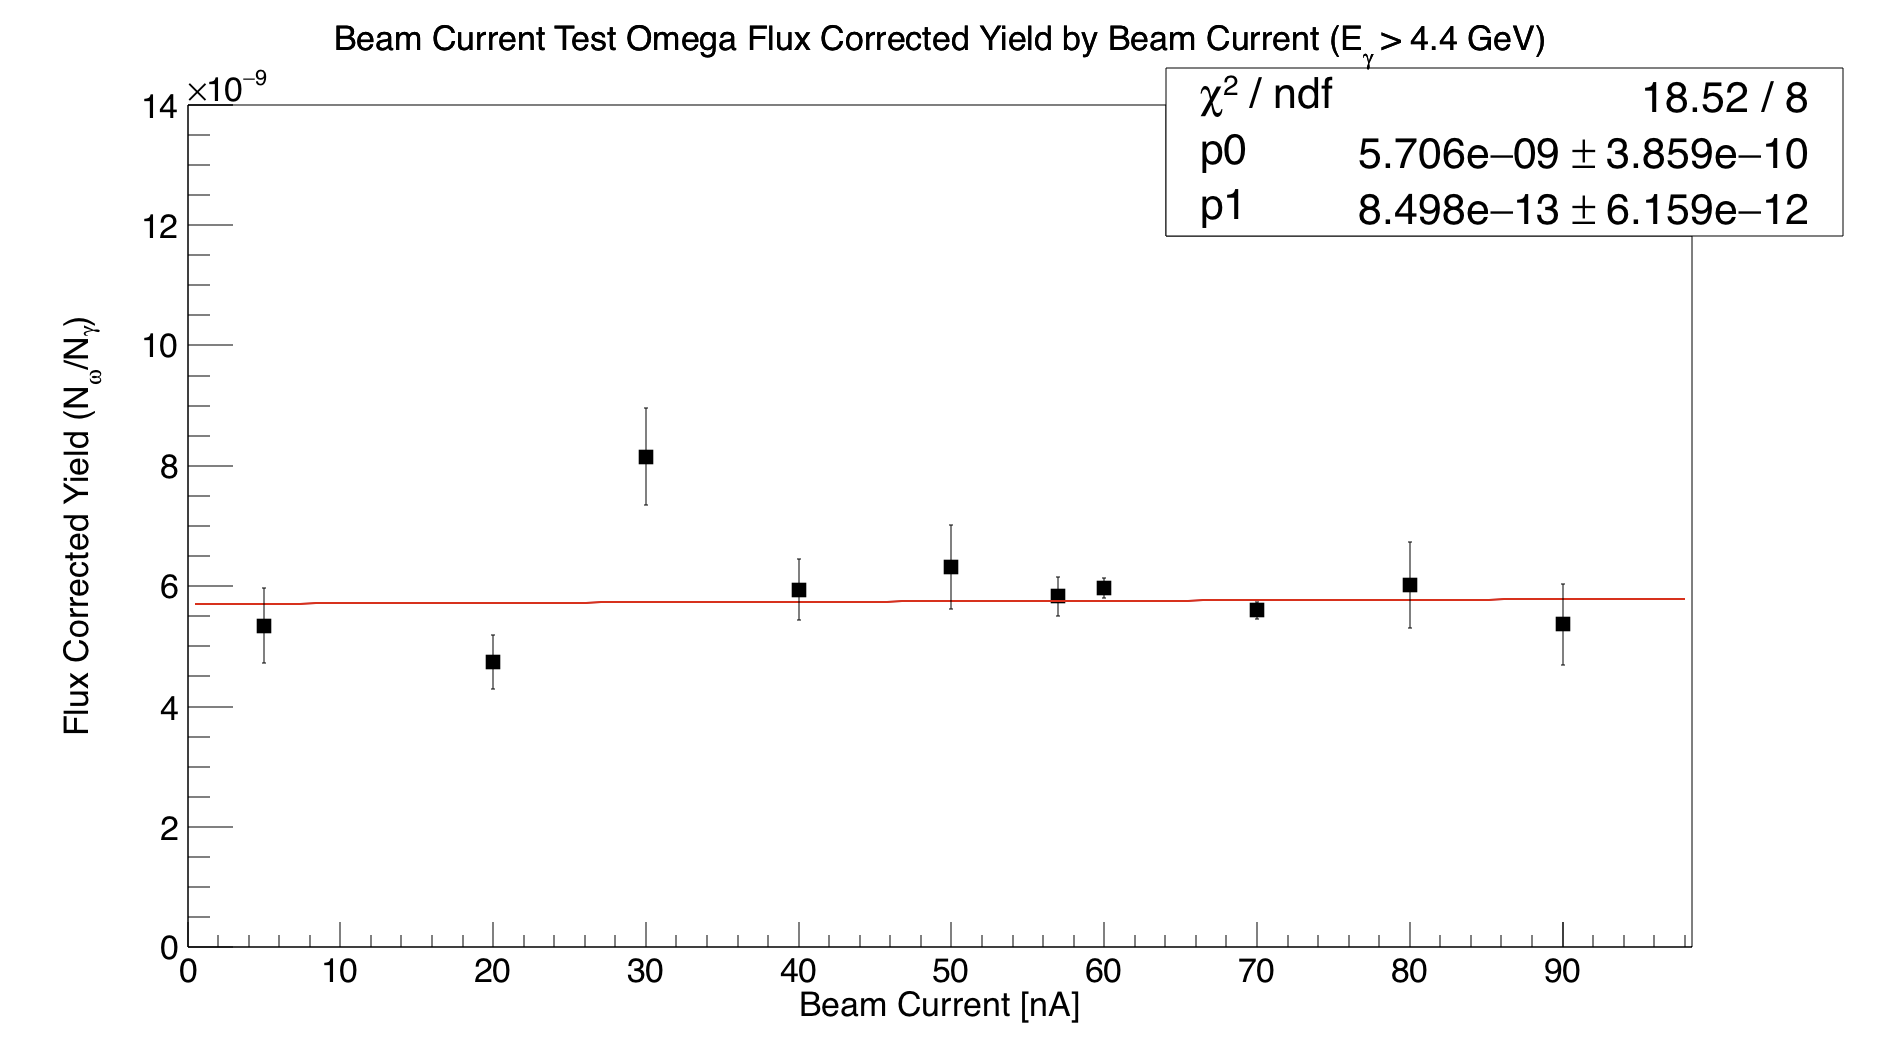
\includegraphics[width=0.6\columnwidth]{{figures/xsec/omegaYieldsCurrent}.png}
\caption[]{\label{fig:omega.yields}The flux-corrected yield of the ω by beam current for high-energy part of the tagger ($E_\text{γ} > 4.4$~GeV).}
\end{center}\end{figure}


\subsection{\label{sec:flux.runbyrun}Run-by-run Stability and Systematic Uncertainty of Flux}

Fig.~\ref{gfluxbyrun} shows the stability of the flux corrections for runs after run 56519. These runs all use the same trigger and have a cut on $E_{\gamma}$ > 4.4 GeV. \begin{v2}These data were projected onto the $y$-axis and fit to a Gaussian and the resulting error on the mean indicates a systematic uncertainty of 0.5\%, though the width of the fit indicates a statistical uncertainty of approximately 10\%.\end{v2}

\begin{figure}[htpb]
\begin{center}
 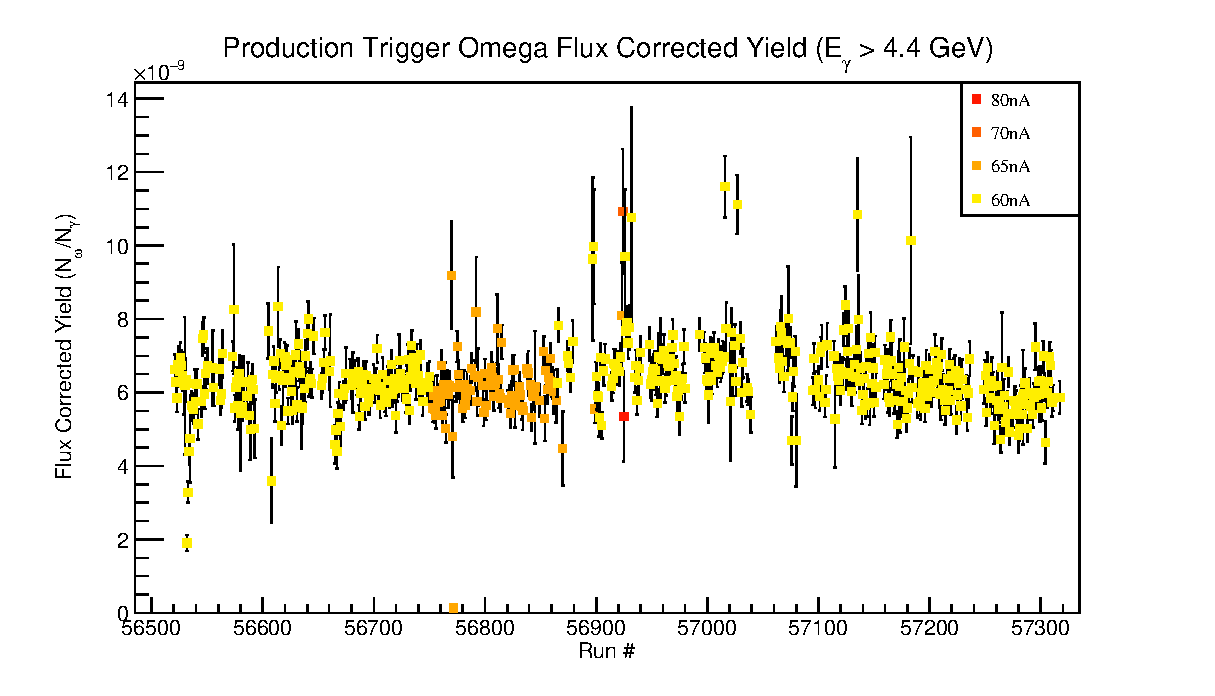
\includegraphics[width=0.9\textwidth]{figures/gflux/gflux_runstability_omega.eps}
  \caption{Photon flux normalized yields by run for the production runs (Runs > 56519).}
  \label{gfluxbyrun}
  \end{center}
\end{figure}

\begin{figure}[htpb]
\begin{center}
 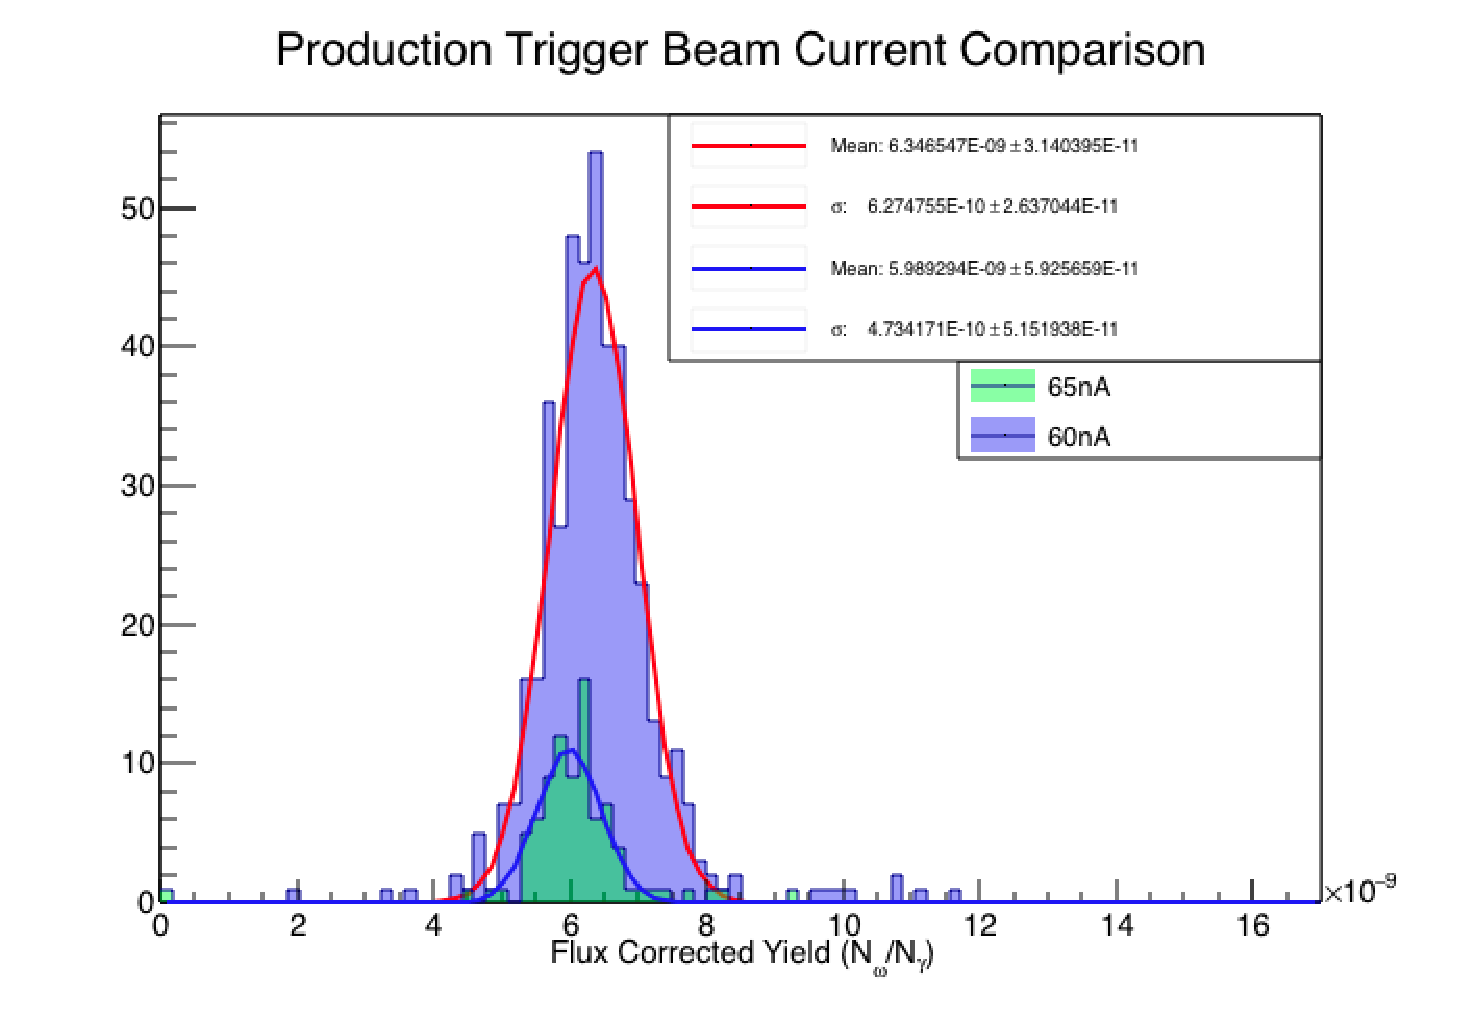
\includegraphics[width=0.9\textwidth]{figures/gflux/60vs65comparison_withparameters.eps}
  \caption{Gaussian fit to 60 and 65~nA data shown in Fig.~\ref{gfluxbyrun}. The error on the mean indicates a systematic uncertainty of 0.5\%. The sigma of the Gaussian fit indicates a statistical uncertainty of approximately 10\%.}
  \label{gfluxbyrun_pull}
  \end{center}
\end{figure}

\begin{v2}
The algorithm for summing the flux in each energy bin in \prog{g12-gflux} is rather crude. It locks each energy bin to the center-point energy of the 767 tagger (logical) paddles. If finer control over the binning is required, one may use the \prog{g12-gflux-all} program to return the flux in each individual logical energy bin of the tagger.

There are two regions in the tagger that should be cut out of any analysis - in data, simulation and flux. The photon energy ranges affected are:
\begin{eqnarray}
    E_\text{γ} &\in [2.975,3.175], \\ \nonumber
    E_\text{γ} &\in [3.475,3.575].
\end{eqnarray}
The first is due to a bad paddle readout (possibly a dead PMT), and the second is due to missing flux information.
\end{v2}
The width of the normalized yields distributions for given intensity in fact is consistent with the expected statistical widths. In Fig.~\ref{gfluxbyrun_pull}, one can see that the widths are 6.2E-10 (60nA) and 4.7E-10(65nA). The expected statistical width (shown in Fig.~\ref{gfluxbyrun_uncertain}) are actually 4.9E-10 (60nA, RMS: 2.6E-10) and 4.8E-10(65nA, RMS: 2.9E-10). These are consistent with each other and we should stick to the currently quoted lower bound of the systematic uncertainty for the g12 normalization of 5.7%. 
\begin{figure}[htpb]
	\begin{center}
		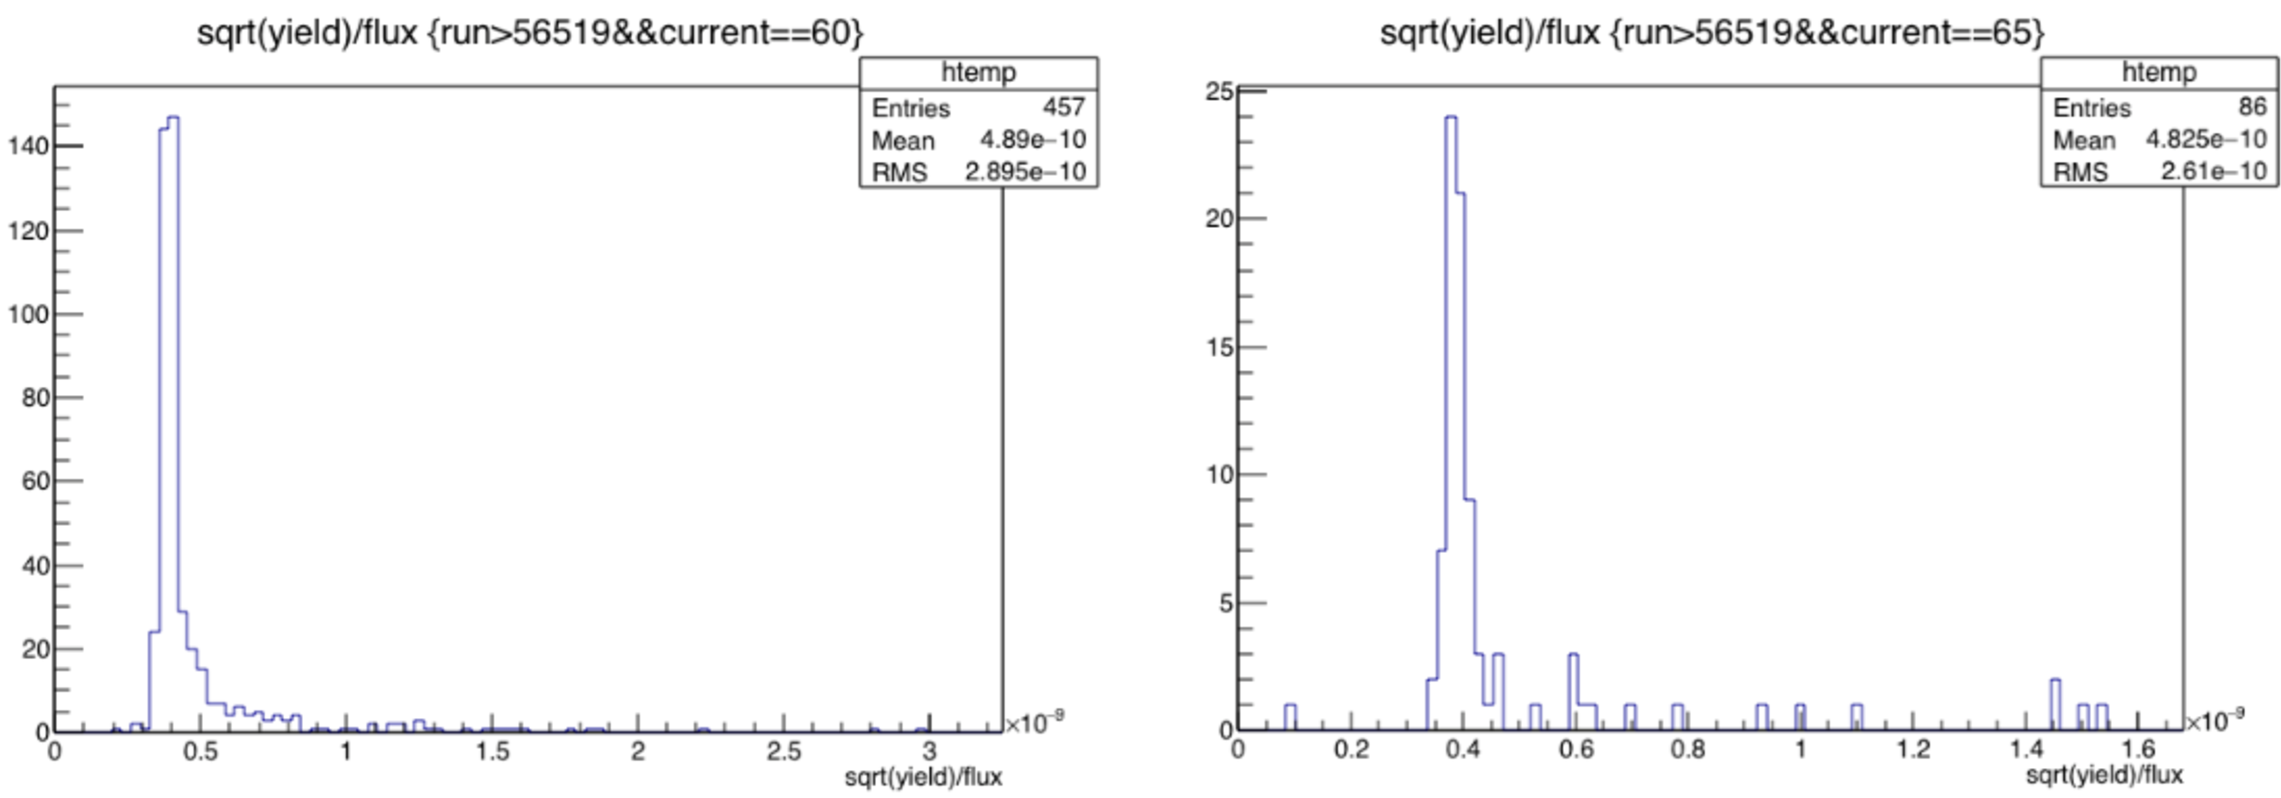
\includegraphics[width=0.9\textwidth]{figures/gflux/gflux_uncertaintiy.ps}
		\caption{Expected statistical uncertainty for the flux normalized omega yields, for 60nA runs (left) and 65nA runs (right).}
		\label{gfluxbyrun_uncertain}
	\end{center}
\end{figure}
\FloatBarrier
